\section{Теория}
\subsection{Подсчет контуров, узлов  и ветвей}
\begin{figure}[H]
    \centering
    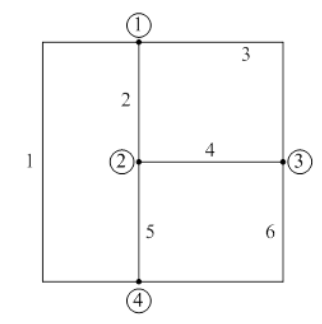
\includegraphics[width=0.4\textwidth]{images/image_1_contures_nodes_branches.png}
    \caption{Граф электрической цепи}
    \label{fig:graph}
\end{figure}

\textbf{Граф цепи} - скелетная форма цепи, состоящая только из ветвей и узлов, соединяющих их. По сути это соединения проводников без участия элементов цепи. Такой граф показывает как может проходить электрический ток. Как правило, в больших электрических схемах оказывается полезным превращать электрическую схему в граф для того, чтобы уменьшить нагромождения и посчитать количество узлов, ветвей и контуров.

\textbf{Ветвь графа цепи} - такой элемент графа по которому протекает один и тот же ток, т.е. элемент является неразрывным проводником, не содержащим внутри себя узел. Обычно, ветвь образуется между двумя узлами. Ветвь может содержать сразу несколько как пассивных, так и активных элементов

На рисунке \ref{fig:graph2} показаны 6 ветвей.

\begin{figure}[H]
    \centering
    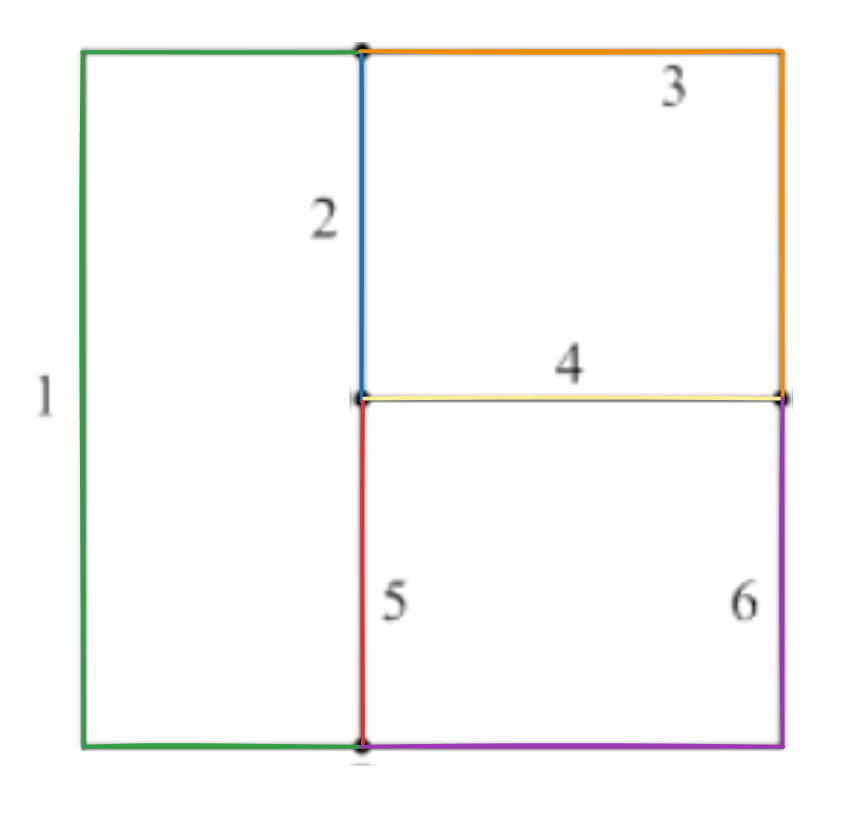
\includegraphics[width=0.4\textwidth]{images/image_2_contures_nodes_branches.png}
    \caption{Ветви графа электрической цепи}
    \label{fig:graph2}
\end{figure}

Узел графа - место соединения трех или более ветвей . Является началом или концом ветви. 

На рисунке \ref{fig:graph3} показаны 4 узла.

\begin{figure}[H]
    \centering
    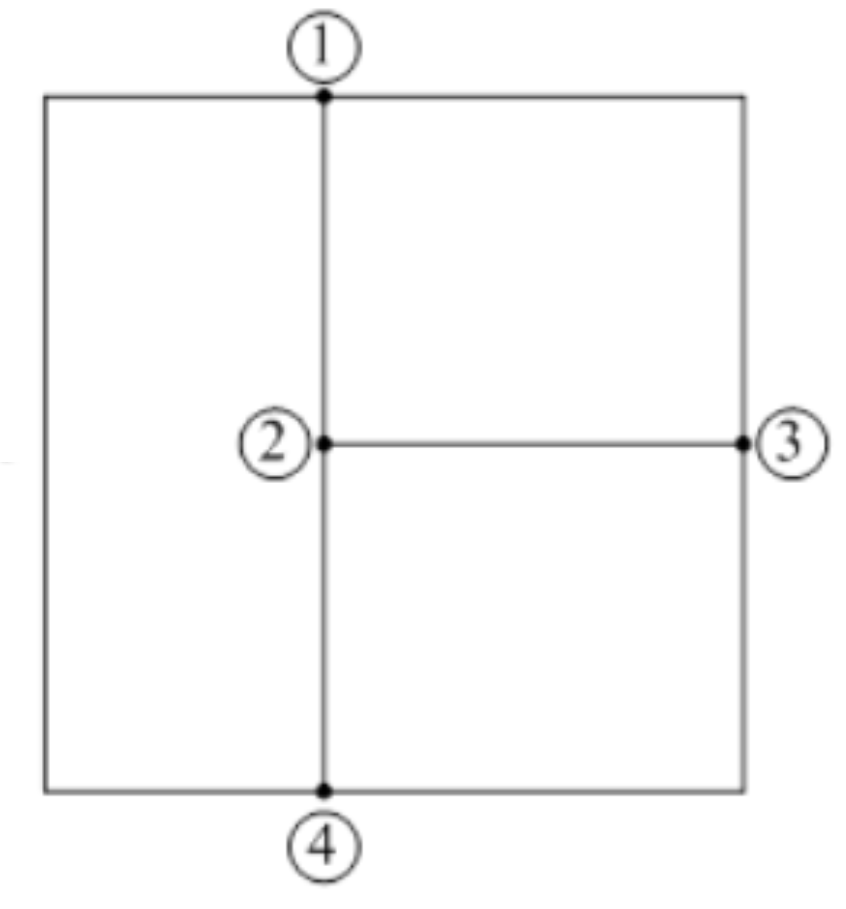
\includegraphics[width=0.4\textwidth]{images/image_3_contures_nodes_branches.png}
    \caption{Узлы графа электрической цепи}
    \label{fig:graph3}
\end{figure}

Контур графа цепи - замкнутый путь, который состоит из ветвей графа, соединенных узлами.

На рисунке \ref{fig:graph4} показаны 7 контуров

\begin{figure}[H]
    \centering
    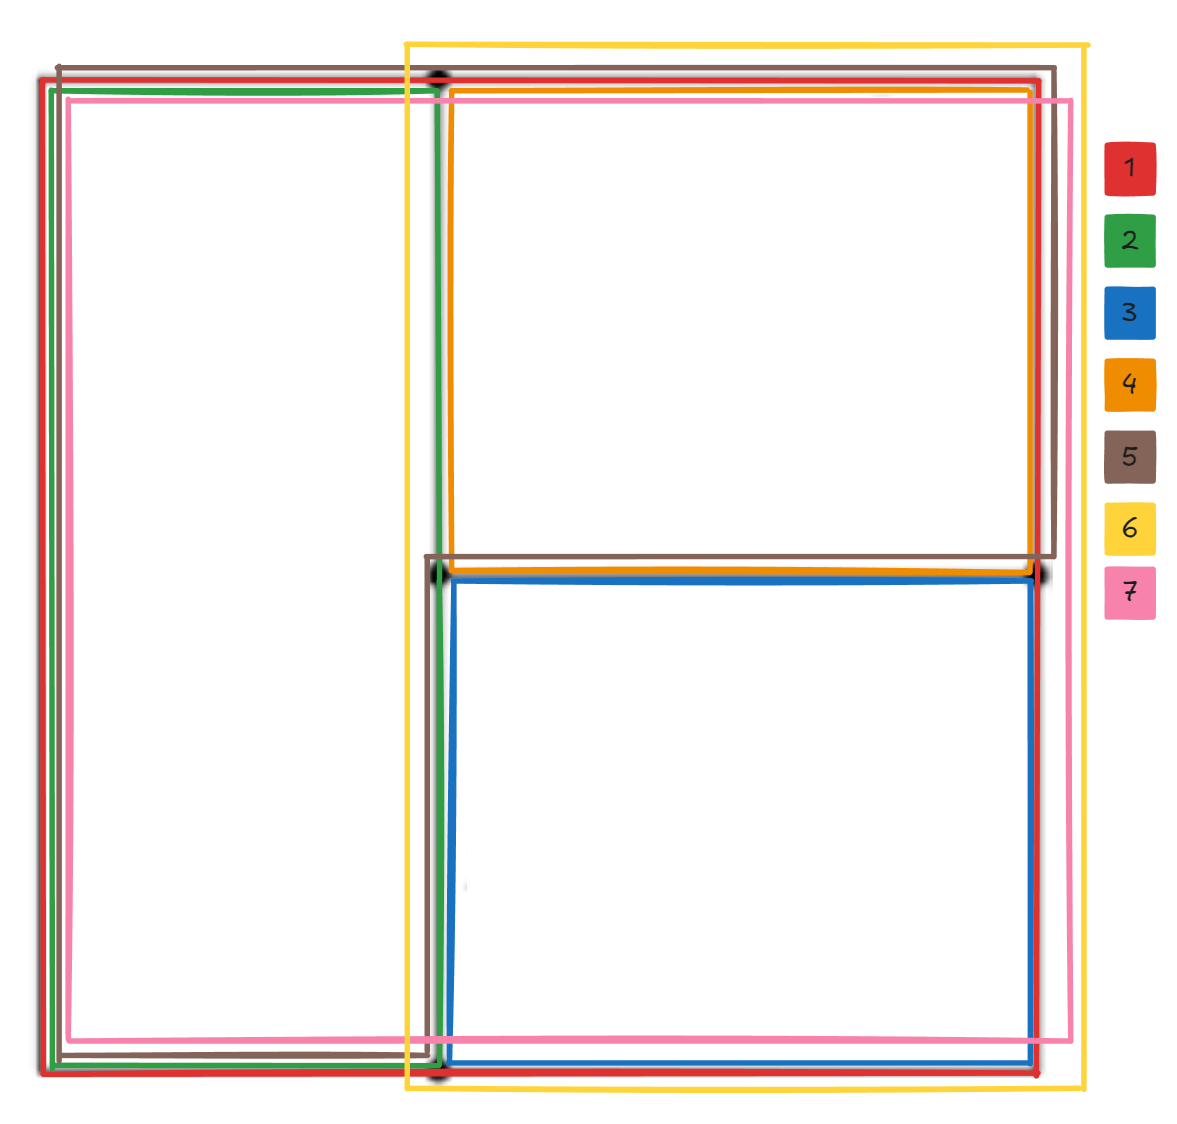
\includegraphics[width=0.4\textwidth]{images/image_4_contures_nodes_branches.png}
    \caption{Узлы графа электрической цепи}
    \label{fig:graph4}
\end{figure}

Независимые контура цепи - такие контура цепи, имеющие **только одну** ветвь входящую в множество ветвей, образующую этот контур 

Понятие независимости контуров является свойством, которое описывает взаимоотношения нескольких контуров, но не одного. Поэтому независимым может быть только контур 1 по отношению к контуру 2, сам по себе контур 1 не может быть независимым

На рисунке \ref{fig:graph5} контур 1 является независимым по отношению к 2 и 3, однако это не единственная комбинация независимых контуров.

\begin{figure}[H]
    \centering
    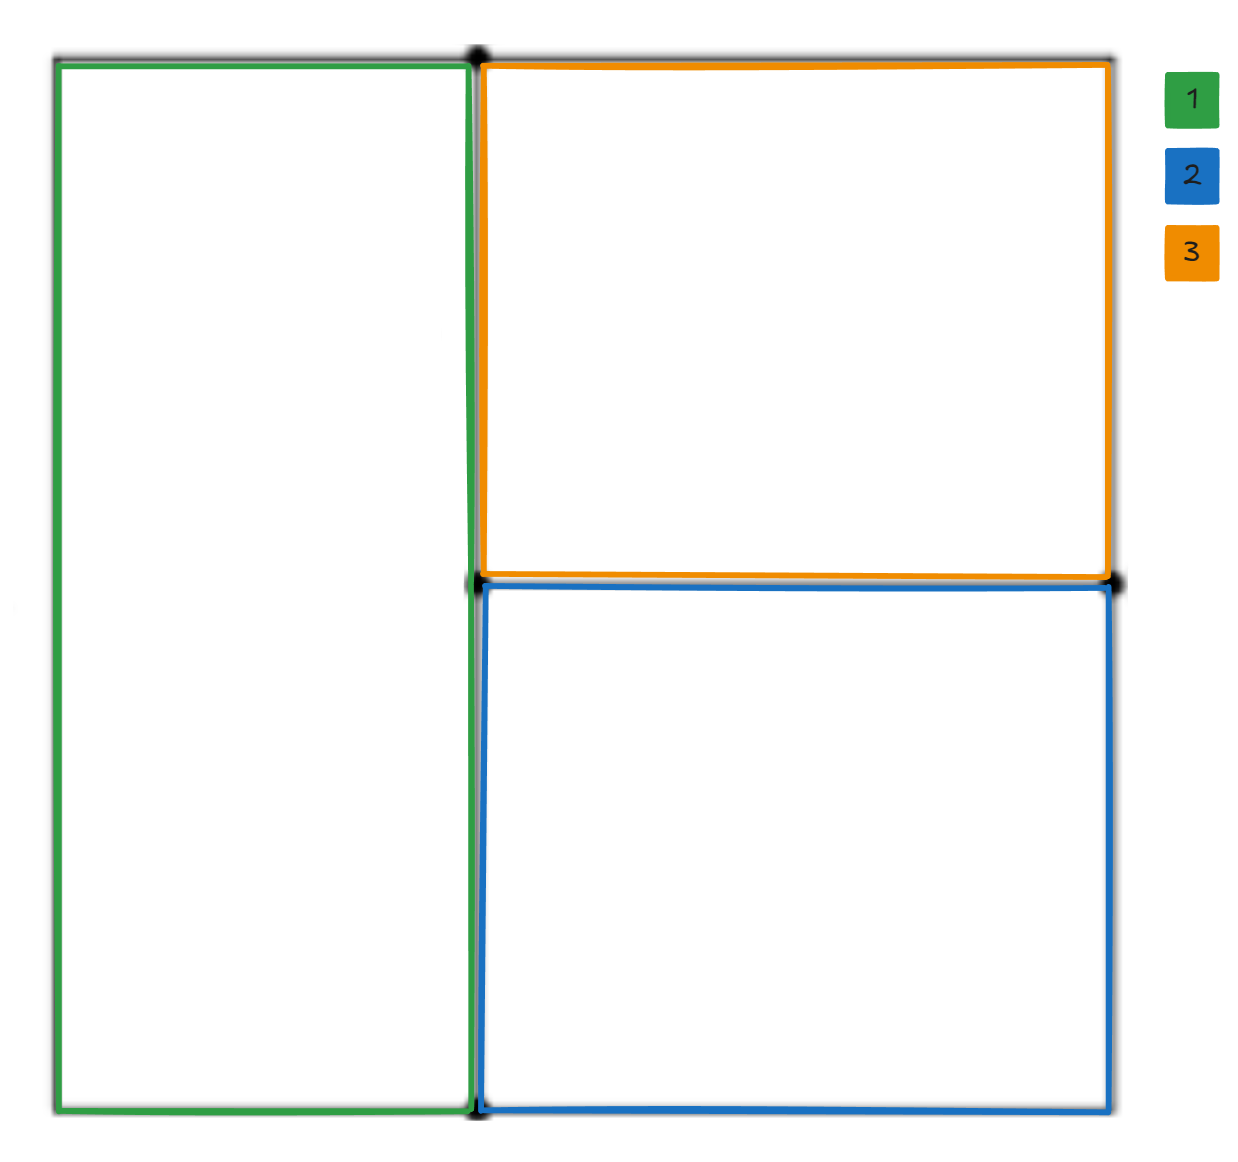
\includegraphics[width=0.4\textwidth]{images/image_5_contures_nodes_branches.png}
    \caption{Независимые контура графа электрической цепи}
    \label{fig:graph5}
\end{figure}

\subsection{Закон Ома и уравнение Джоуля Ленца}

\textbf{Закон Ома} - это закон, который связывает напряжение, ток и сопротивление в электрической цепи. Технически, закон Ома является математическим описанием пассивного элемента цепи - электрического сопротивления.

\begin{figure}[H]
    \centering
    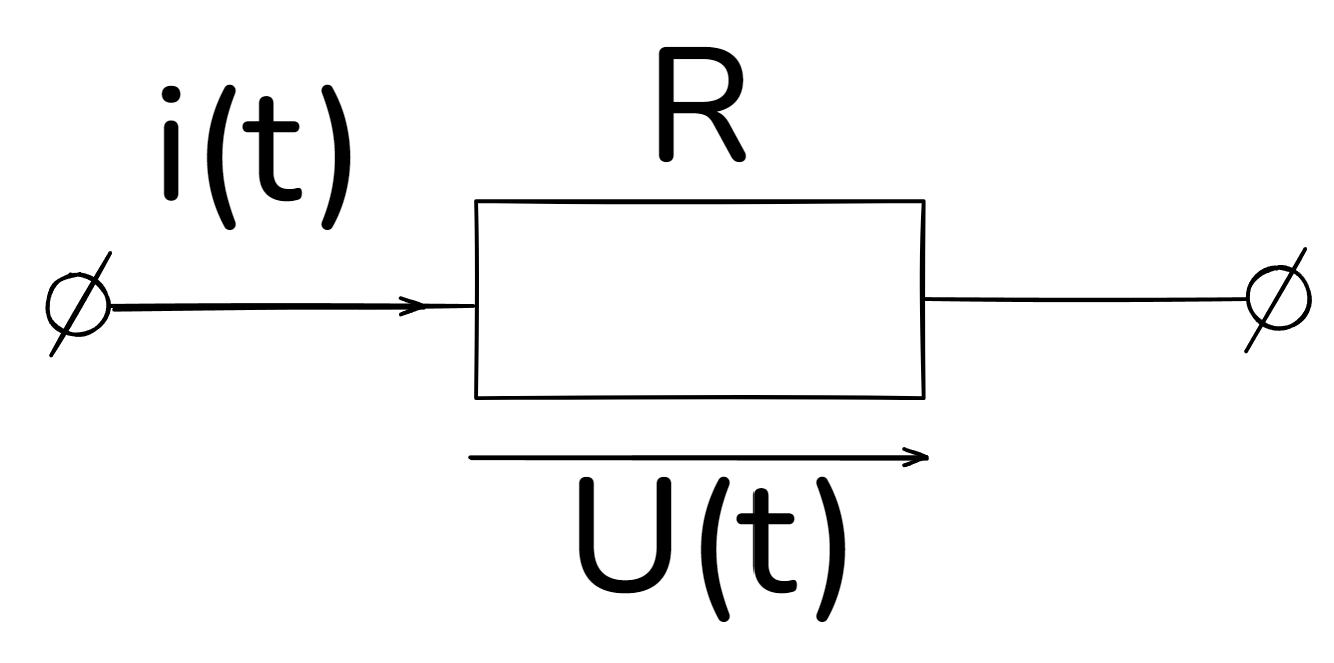
\includegraphics[width=0.4\textwidth]{images/image_1_ohm_laws_power.png}
    \caption{Закон Ома для неполной цепи}
    \label{fig:graph6}
\end{figure}

Закон Ома для неполной цепи \ref{fig:graph6} описывает абстрактное понятие напряжение и записывается следующим образом (\ref{eq:ohms_law}):
\begin{equation}
    I = \frac{U}{R}
    \label{eq:ohms_law}
\end{equation}

где $U$ - напряжение, $I$ - ток, $R$ - сопротивление.

\begin{figure}[H]
    \centering
    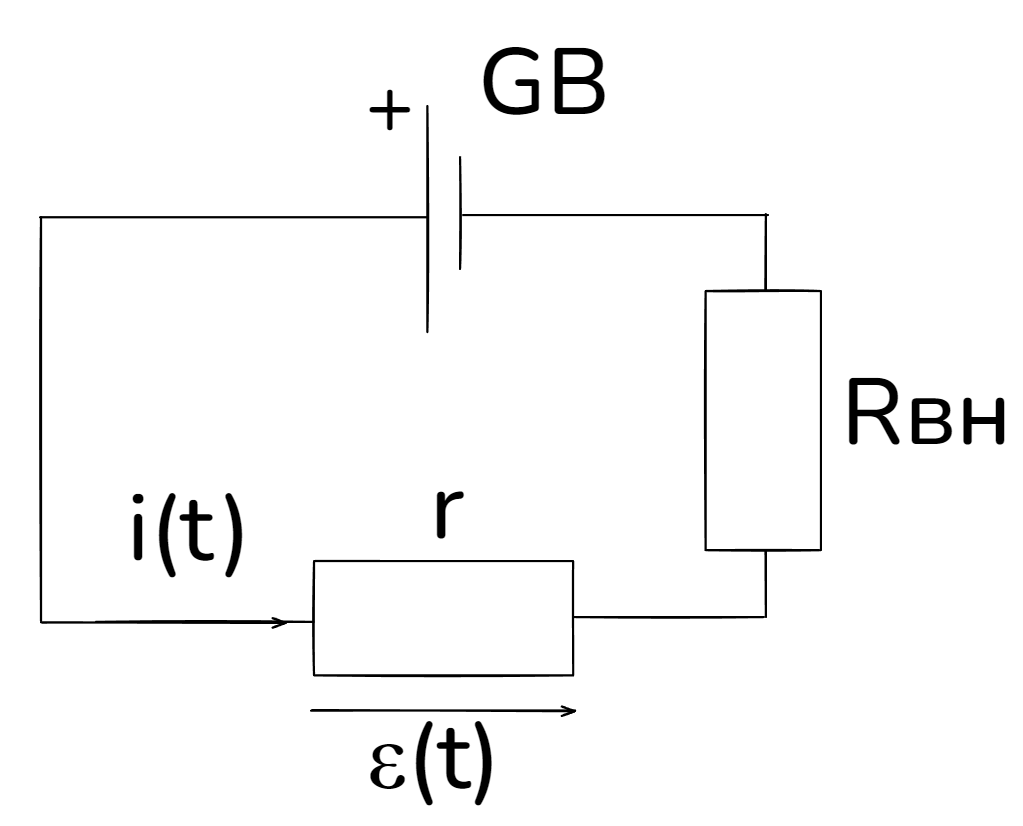
\includegraphics[width=0.4\textwidth]{images/image_2_ohm_laws_power.png}
    \caption{Закон Ома для полной цепи}
    \label{fig:graph7}
\end{figure}

В то время как закон Ома для полной цепи (\ref{fig:graph7}) выражается через понятие ЭДС и учитывает внутреннее сопротивления источника электрического тока. В этом случае полный закон Ома записывается следующим образом (\ref{eq:ohms_law_full}):
\begin{equation}
    I = \frac{\mathcal{E}}{R + r}
    \label{eq:ohms_law_full}
\end{equation}

где $\mathcal{E}$ - ЭДС источника, $R$ - внешнее сопротивление, $r$ - внутреннее сопротивление источника.

В пассивных элементах цепи происходит преобразование электрической энергии в другие виды энергии. В контексте пассивного элемента обладающего электрическимсопротивлением, энергия электрического тока преобразуется в тепловую энергию. Этот процесс описывается уравнением Джоуля Ленца (\ref{eq:joule_lenz}):
\begin{equation}
    Q = I^2 R t
    \label{eq:joule_lenz}
\end{equation}

где $Q$ - количество теплоты, $I$ - ток, $R$ - сопротивление, $t$ - время.

\subsection{Последовательное и параллельное соединение. Метод эквивалентных преобразований}
Эквивалетными преобразованиями называют методы расчета простых цепей с использованием закона Ома и преобразований участков схемы. 

Различают два основных типа эквивалетных преобразований: последовательное и параллельное соединение. Кроме того, встречаются нестандартные типы соединения: звезда и треугольник. Существуют методики для перевода этих типов соединения в комбинацию линейных преобразований.

Последовательное соединение резисторов \ref{fig:graph8} описывается следующим образом:

\begin{figure}[H]
    \centering
    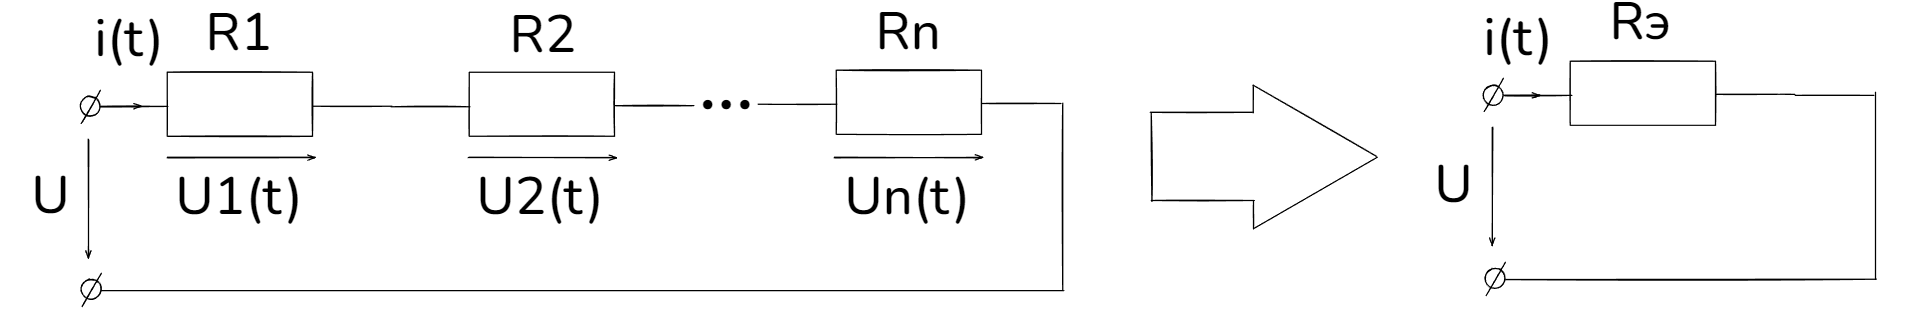
\includegraphics[width=1\textwidth]{images/image_1_resistor_merge.png}
    \caption{Последовательное соединение резисторов}
    \label{fig:graph8}
\end{figure}

При последовательном соединении резисторов через них протекает один и тот же ток (это следует как из закона Ома для неполной цепи, так и из того факта, что все резисторы находятся на одной ветви), однако на каждом из элементов падает напряжение, которое зависит от значения сопротивления. Сумма падений напряжений на всех сопротивлениях равна напряжению на всем участке цепи.

\begin{equation}
    R = R_1 + R_2 + \cdots + R_n
    \label{eq:resistor_merge_series}
\end{equation}

\begin{figure}[H]
    \centering
    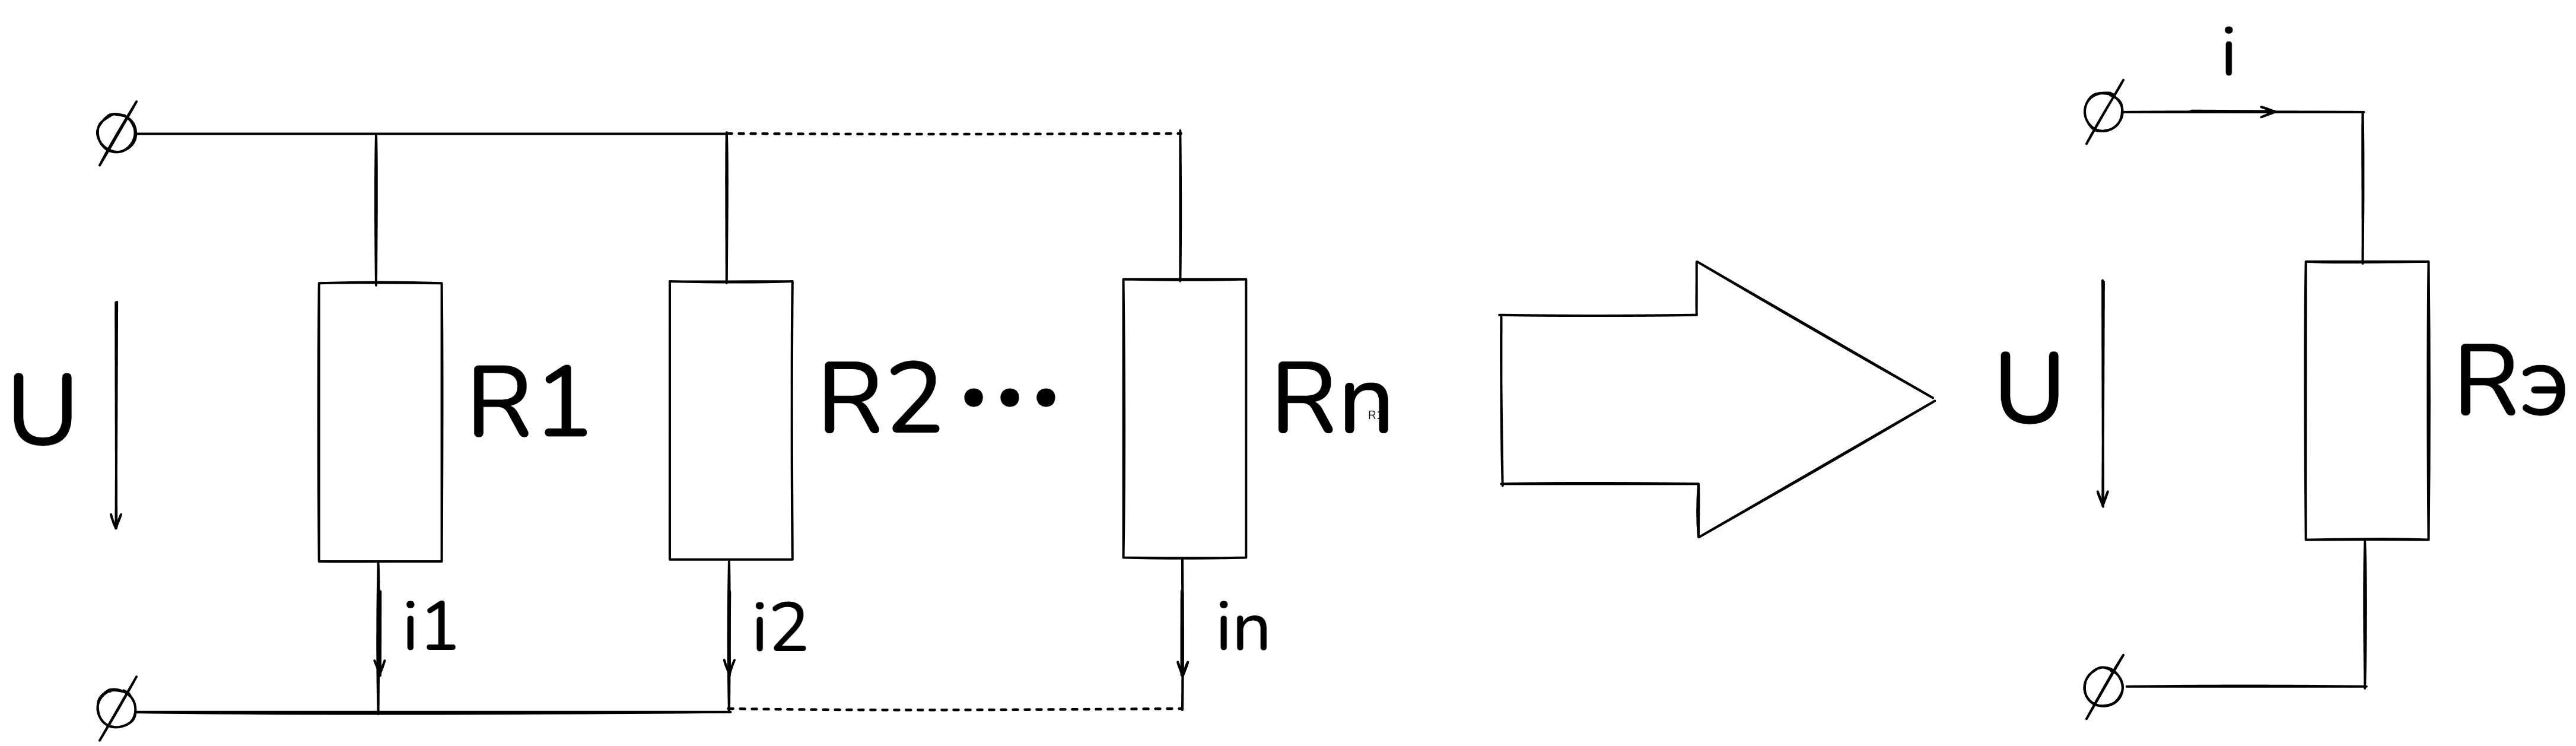
\includegraphics[width=0.7\textwidth]{images/image_2_resistor_merge.png}
    \caption{Параллельное соединение резисторов}
    \label{fig:graph9}
\end{figure}

При параллельном соединении резисторов через них протекает ток, который зависит от значения сопротивления. Сумма токов через все сопротивления равна току на всем участке цепи. При этом напряжение на всех сопротивлениях одинаковое.

\begin{equation}
    \frac{1}{R} = \frac{1}{R_1} + \frac{1}{R_2} + \cdots + \frac{1}{R_n}
    \label{eq:resistor_merge_parallel}
\end{equation}


\subsection{Решение задач в линейных цепях постоянного тока}

\subsubsection{Формулировка проблемы}
Обычно в задачах на расчет цепей постоянного тока требуется найти токи, напряжения и мощности на всех элементах цепи, но наиболее часто задача сводится именно к определению токов в ветвях.
Дано: электрическая цепь, состоящая из нескольких пассивных и активных элементов, соединенных между собой определенным образом, значения элементов цепи как активных так и пассивных (сопротивления, емкости индуктивности, напряжения и токи источников).
Найти: токи в ветвях.


\subsubsection{Законы Кирхгофа}
Наиболее классическим методом решения задач на расчет цепей постоянного тока является метод основанный на законах Кирхгофа.
Первый закон Кирхгофа звучит следующим образом:

\begin{tcolorbox}[
    colback=blue!5!white,
    colframe=black!50!black,
    title=Первый закон Кирхгофа,
    fonttitle=\bfseries,
    arc=3pt,
    boxrule=1pt
]
Алгебраическая сумма токов входящих в узел равна алгебраической сумме токов выходящих из узла.
\end{tcolorbox}
\begin{equation}
    \sum_{i=1}^{n} I_i^{\text{вх}} = \sum_{i=1}^{n} I_i^{\text{вых}},
    \label{eq:kirchhoff_laws_1}
\end{equation}
где $I_i^{\text{вх}}$ - ток входящий в узел, $I_i^{\text{вых}}$ - ток выходящий из узла.

Второй закон Кирхгофа звучит следующим образом:

\begin{tcolorbox}[
    colback=blue!5!white,
    colframe=black!50!black,
    title=Второй закон Кирхгофа,
    fonttitle=\bfseries,
    arc=3pt,
    boxrule=1pt
]
Алгебраическая сумма ЭДС в контуре равна алгебраической сумме падений напряжения на элементах в этом контуре.
\end{tcolorbox}

\begin{equation}
    \sum_{i=1}^{n} \mathcal{E}_i = \sum_{i=1}^{n} U_i,
    \label{eq:kirchhoff_laws_2}
\end{equation}
где $\mathcal{E}_i$ - ЭДС источника, $U_i$ - падение напряжения на элементе.

В свою очередь падение напряжения на элементе определяется в зависимости от физического характера элемента.

В случае электрического сопротивления падение напряжения определяется по закону Ома для неполной цепи:
\begin{equation}
    U_R = I_R R,
    \label{eq:kirchhoff_laws_2_1}
\end{equation}
где $I_R$ - ток через резистор, $R$ - сопротивление резистора.

В случае электрической емкости падение напряжения определяется как интеграл от тока через элемент:
\begin{equation}
    U_C = \frac{1}{C} \int_{0}^{t} I_C dt,
    \label{eq:kirchhoff_laws_2_2}
\end{equation}
где $C$ - емкость конденсатора, $I_C$ - ток через конденсатор, $t$ - время.

В случае электрической индуктивности падение напряжения определяется как дифференциал от тока через элемент:
\begin{equation}
    U_L = L \frac{dI_L}{dt},
    \label{eq:kirchhoff_laws_2_3}
\end{equation}
где $L$ - индуктивность катушки, $I_L$ - ток через катушку, $t$ - время.

Сложные цепи постоянного тока имеют количество источников более одного и более широкий класс соединений элементов цепи. При расчете сложных ЭЦ универсальным является метод расчета по законам Кирхгофа. Расчет таких цепей следует начинать с произвольного выбора стрелок токов в ветвях ЭЦ.

Количество расчетных уравнений Кирхгофа должно совпадать с количеством неизвестных токов схемы. Полученная система расчетных уравнений должна быть линейно независимой. Для этого уравнения Кирхгофа должны составляться для независимых узлов и независимых контуров.

\begin{tcolorbox}[
    colback=black!5!white,
    colframe=black!50!black,
    title=Алгоритм решения задач методом законов Кирхгофа,
    fonttitle=\bfseries,
    arc=3pt,
    boxrule=1pt
]
\begin{enumerate}
    \item Определить количество узлов и ветвей в цепи;
    \item Выбрать независимые контуры;  
    \item Выбрать направления токов в ветвях и направления обхода контуров;
    \item Записать уравнения для узлов и контуров;
    \item Решить систему алгебраических уравнений;
    \item Найти токи в ветвях;
    \item Найти напряжения на элементах цепи;
    \item Найти мощности на элементах цепи.
\end{enumerate}
\end{tcolorbox}

Для сложных ЭЦ, как правило, количество этих уравнений достаточно велико и их решение вручную весьма затруднительно. При современном уровне вычислительной техники расчеты проводятся на ЭВМ, однако составление уравнений долгая и утомительная работа.


\subsubsection{Метод контурных токов}

На ранних этапах развития расчетных методов были созданы косвенные методы снижающие порядок решаемых уравнений Кирхгофа. Характерным для косвенных методов анализа является то, что в уравнениях, описывающих электромагнитное состояние ЭЦ, в качестве переменных подлежащих определению, выступают не искомые токи и напряжения, а некоторые вспомогательные величины, например, узловые потенциалы и контурные токи.


Метод контурных токов является одним из основных косвенных методов расчета ЭЦ, который находит широкое применение на практике. Сущность этого метода заключается в том, что в каждом независимом контуре протекает свой условный, так называемый «контурный» ток. Система уравнений для контурных токов получается как результат сведения законов Кирхгофа к уравнениям только для независимых контуров.


\begin{tcolorbox}[
    colback=black!5!white,
    colframe=black!50!black,
    title=Порядок расчета методом контурных токов,
    fonttitle=\bfseries,
    arc=3pt,
    boxrule=1pt
]
\begin{enumerate}
    \item Определяем независимые контуры и указываем направления отсчета контурных токов и действительных токов в ветвях;
    \item Определяем собственные, смежные сопротивления контуров и контурные ЭДС контуров;
    \item Составляем уравнения для контурных токов, используя стандартную форму записи этих уравнений. Решаем полученную систему уравнений и определяем контурные токи ЭЦ;
    \item Действительные токи определяются как алгебраическая сумма контурных токов, протекающих в этой ветви.
\end{enumerate}
\end{tcolorbox}

Действительный ток ветви находится как алгебраическая сумма контурных токов, протекающих в этой ветви. При этом, если направление действительного тока совпадает с направлением контурного тока, то контурный ток берется с собственным знаком. В противном случае контурный ток берется с противоположным знаком.

\subsubsection{Метод узловых потенциалов}


Методом узловых потенциалов называют метод анализа электрических цепей, в которых неизвестными являются потенциалы узлов ЭЦ. Потенциал одного из узлов называемого базисным принимается равным нулю. В качестве базисного узла схем обычно выбирают узел, в котором соединяется наибольшее количество элементов или, при наличии в схеме идеальных источников напряжения, узел, с которым соединяется один из зажимов идеального источника напряжения.


Система уравнений для узловых потенциалов получается сведением системы уравнений Кирхгофа к уравнениям только для независимых узлов ЭЦ. Таким образом размерность решаемой системы уравнений уменьшается, что и является основным достоинством косвенных методов расчета ЭЦ.

\begin{tcolorbox}[
    colback=black!5!white,
    colframe=black!50!black,
    title=Последовательность решения задач методом узловых потенциалов,
    fonttitle=\bfseries,
    arc=3pt,
    boxrule=1pt
]
\begin{enumerate}
    \item Определение количества независимых узлов и выбор направлений отсчета искомых токов в ветвях;
    \item Выбор базисного узла;
    \item Составление системы уравнений для узловых потенциалов;
    \item Определение собственных и смежных проводимостей узлов и узловых токов ЭЦ;
    \item Решение системы линейных алгебраических уравнений и определение узловых потенциалов;
    \item Расчет токов в ветвях ЭЦ с использованием рассчитанных узловых потенциалов и законов Кирхгофа и Ома.
\end{enumerate}
\end{tcolorbox}

Токи в ветвях схемы находятся через узловые напряжения по следующему мнемоническому правилу: 

Ток в ветви равен разности узлового потенциала узла из которого он выходит минус узловой потенциал узла в который он входит, плюс ЭДС источника находящегося в этой ветви, если его стрелка совпадает со стрелкой тока или минус ЭДС источника, если его стрелка не совпадает со стрелкой тока и деленное на сопротивление ветви.
\begin{equation}
    I_i = \frac{\varphi_i - \varphi_j + \mathcal{E}_i}{R_i},
    \label{eq:kirchhoff_laws_2_4}
\end{equation}
где $\varphi_i$ - узловой потенциал узла из которого ток выходит, $\varphi_j$ - узловой потенциал узла в который ток входит, $\mathcal{E}_i$ - ЭДС источника находящегося в этой ветви, $R_i$ - сопротивление ветви.

\section{Практика}
\subsection{Варианты заданий}

\begin{table}[H]
\centering
\caption{Параметры источников и элементов}
\begin{tabular}{|c|c|c|c|c|c|c|c|c|c|}
\hline
\multirow{2}{*}{No} & \multicolumn{3}{c|}{\textbf{Источники}} & \multicolumn{6}{c|}{\textbf{Элементы}} \\
\cline{2-4}\cline{5-10}
& $E_1$, В & $E_2$, В & $J$, А & $R_1$, Ом & $R_2$, Ом & $R_3$, Ом & $R_4$, Ом & $R_5$, Ом & $R_6$, Ом \\
\hline
1 & 40 & 20 & 4 & 5 & 2 & 10 & 5 & 6 & 8 \\
2 & 20 & 40 & 2 & 2 & 1 & 30 & 10 & 10 & 2 \\
3 & 40 & 10 & 6 & 4 & 5 & 3 & 3 & 4 & 2 \\
4 & 10 & 40 & 8 & 6 & 3 & 5 & 5 & 10 & 5 \\
5 & 50 & 20 & 1 & 2 & 1 & 30 & 10 & 10 & 2 \\
\hline
6 & 20 & 50 & 3 & 6 & 8 & 5 & 10 & 9 & 4 \\
7 & 60 & 20 & 7 & 4 & 2 & 6 & 6 & 8 & 5 \\
8 & 20 & 60 & 9 & 3 & 1 & 2 & 8 & 10 & 4 \\
9 & 10 & 30 & 5 & 5 & 4 & 1 & 4 & 5 & 8 \\
10 & 30 & 10 & 10 & 3 & 4 & 10 & 4 & 6 & 3 \\
\hline
11 & 10 & 50 & 4 & 6 & 7 & 8 & 6 & 3 & 5 \\
12 & 50 & 10 & 2 & 7 & 8 & 9 & 10 & 5 & 7 \\
13 & 60 & 10 & 6 & 6 & 7 & 10 & 5 & 3 & 2 \\
14 & 10 & 60 & 8 & 7 & 9 & 6 & 10 & 8 & 6 \\
15 & 10 & 70 & 1 & 6 & 8 & 9 & 5 & 7 & 9 \\
\hline
16 & 70 & 10 & 3 & 8 & 9 & 10 & 7 & 5 & 6 \\
17 & 80 & 20 & 7 & 7 & 8 & 6 & 9 & 5 & 10 \\
18 & 20 & 80 & 9 & 6 & 9 & 10 & 5 & 7 & 8 \\
19 & 80 & 10 & 5 & 7 & 8 & 9 & 10 & 5 & 7 \\
20 & 10 & 80 & 10 & 6 & 7 & 9 & 8 & 10 & 8 \\
\hline
\end{tabular}
\label{tab:parameters}
\end{table}

\subsection{Электрические цепи постоянного тока по заданиям}

% Ряд 1: Задачи 1-2
\begin{figure}[H]
    \centering
    \begin{minipage}{0.48\textwidth}
        \centering
        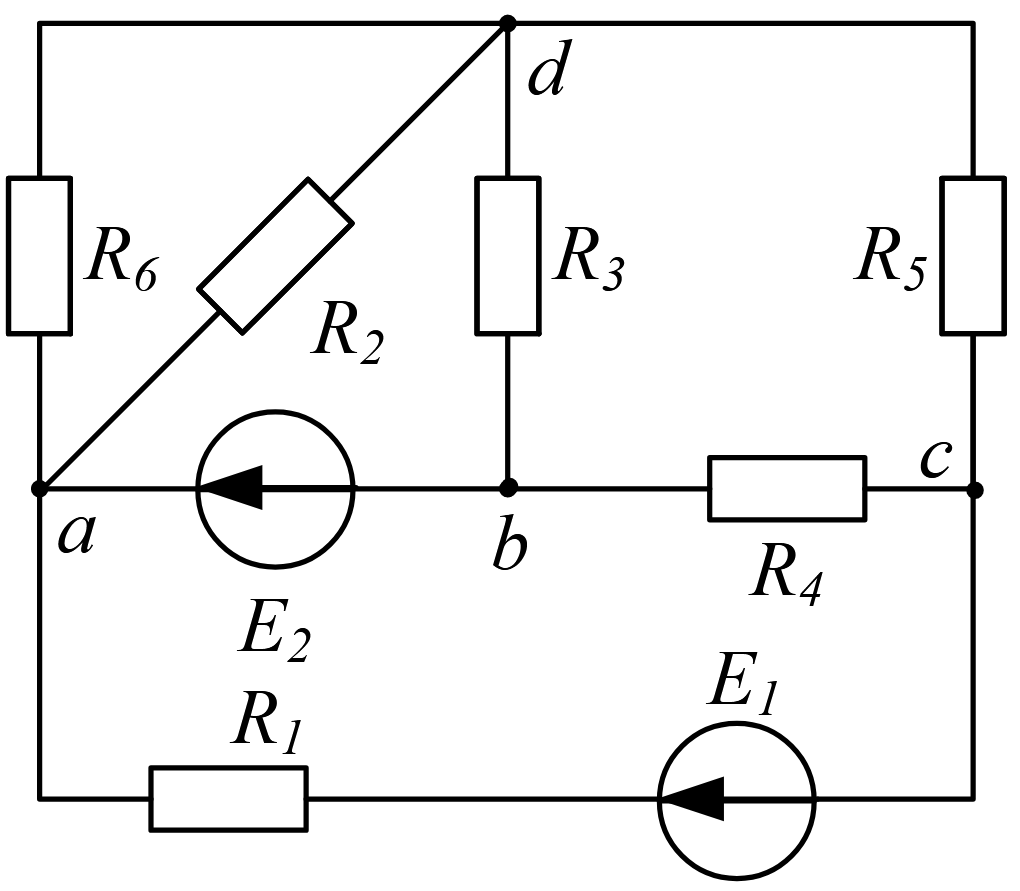
\includegraphics[width=\textwidth]{images/1_task.png}
        \caption{Вариант \#1}
        \label{fig:task_1}
    \end{minipage}
    \hfill
    \begin{minipage}{0.48\textwidth}
        \centering
        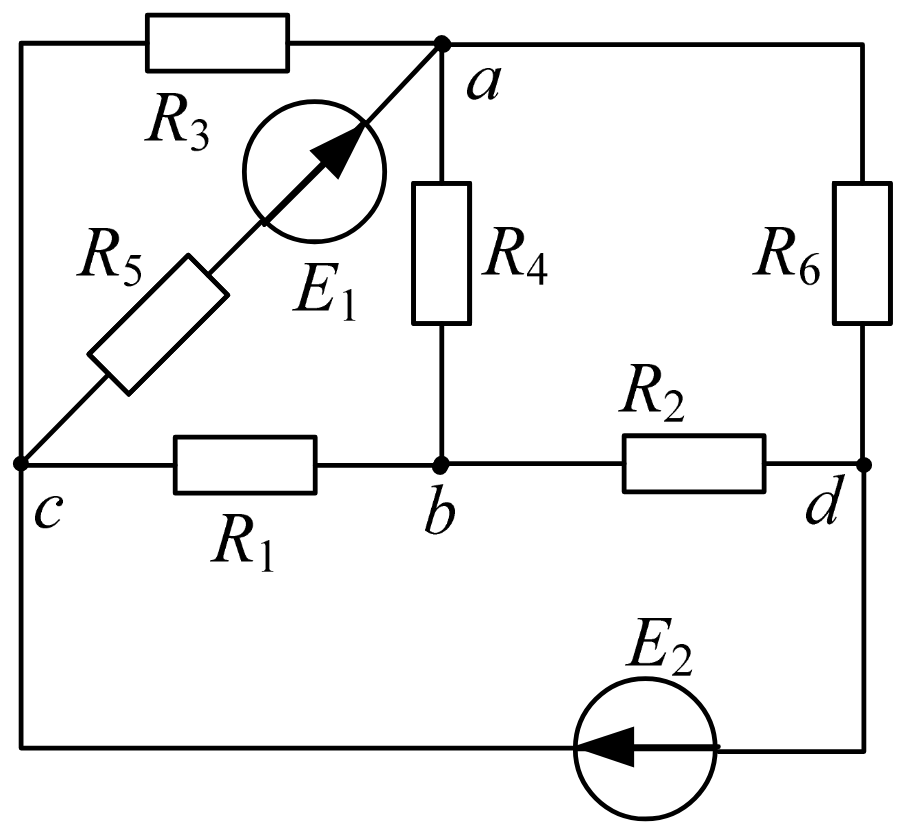
\includegraphics[width=\textwidth]{images/2_task.png}
        \caption{Вариант \#2}
        \label{fig:task_2}
    \end{minipage}
\end{figure}

% Ряд 2: Задачи 3-4
\begin{figure}[H]
    \centering
    \begin{minipage}{0.48\textwidth}
        \centering
        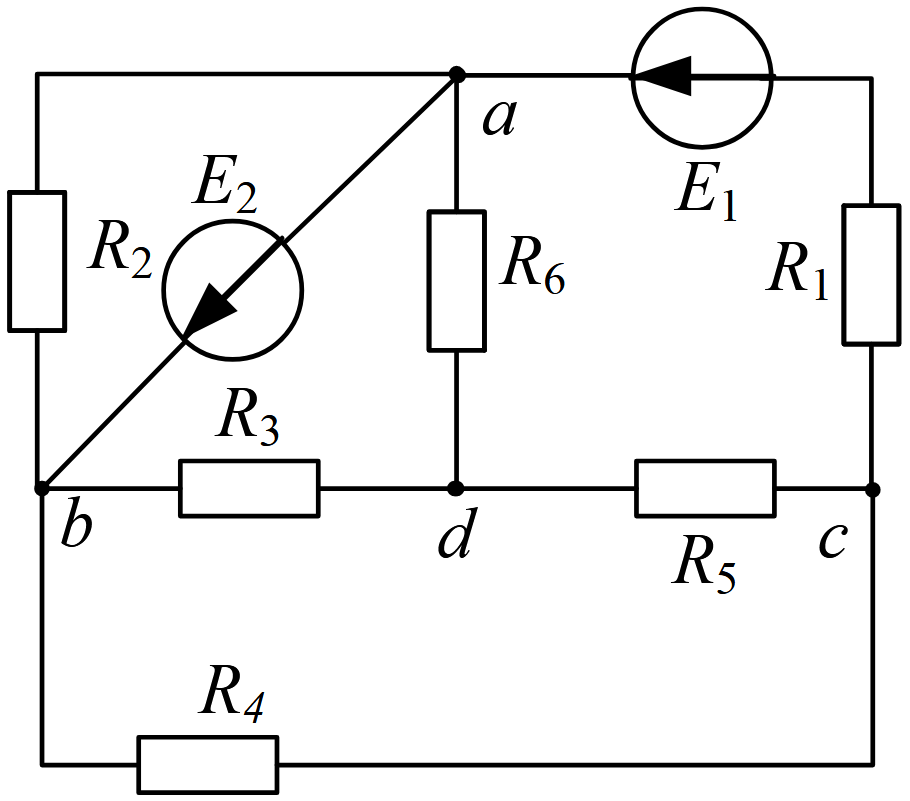
\includegraphics[width=\textwidth]{images/3_task.png}
        \caption{Вариант \#3}
        \label{fig:task_3}
    \end{minipage}
    \hfill
    \begin{minipage}{0.48\textwidth}
        \centering
        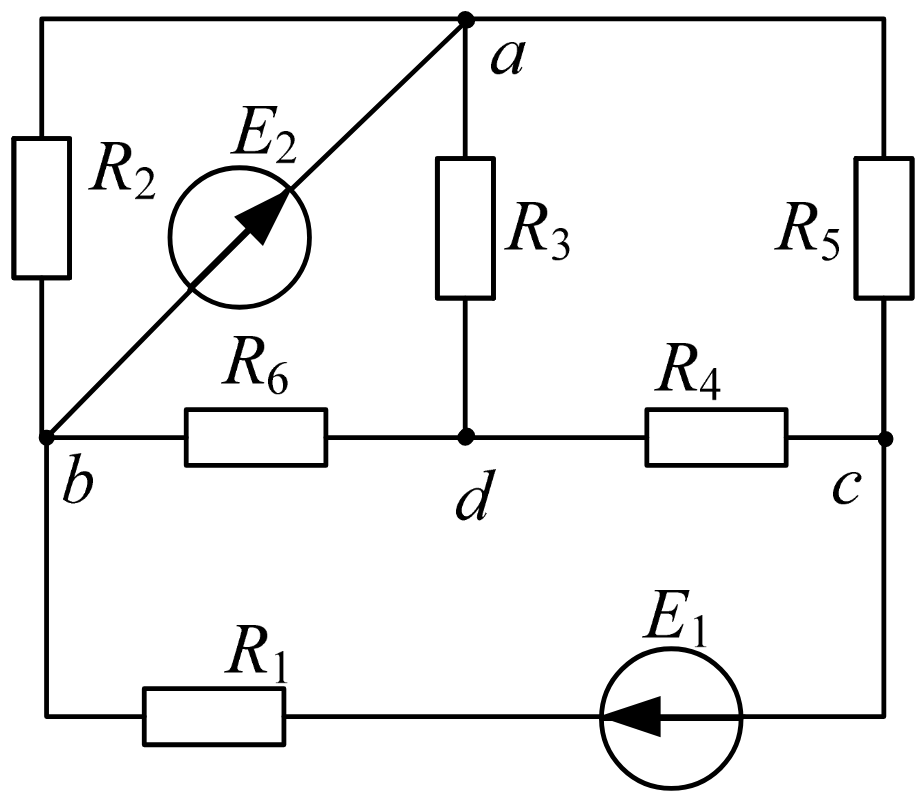
\includegraphics[width=\textwidth]{images/4_task.png}
        \caption{Вариант \#4}
        \label{fig:task_4}
    \end{minipage}
\end{figure}

% Ряд 3: Задачи 5-6
\begin{figure}[H]
    \centering
    \begin{minipage}{0.48\textwidth}
        \centering
        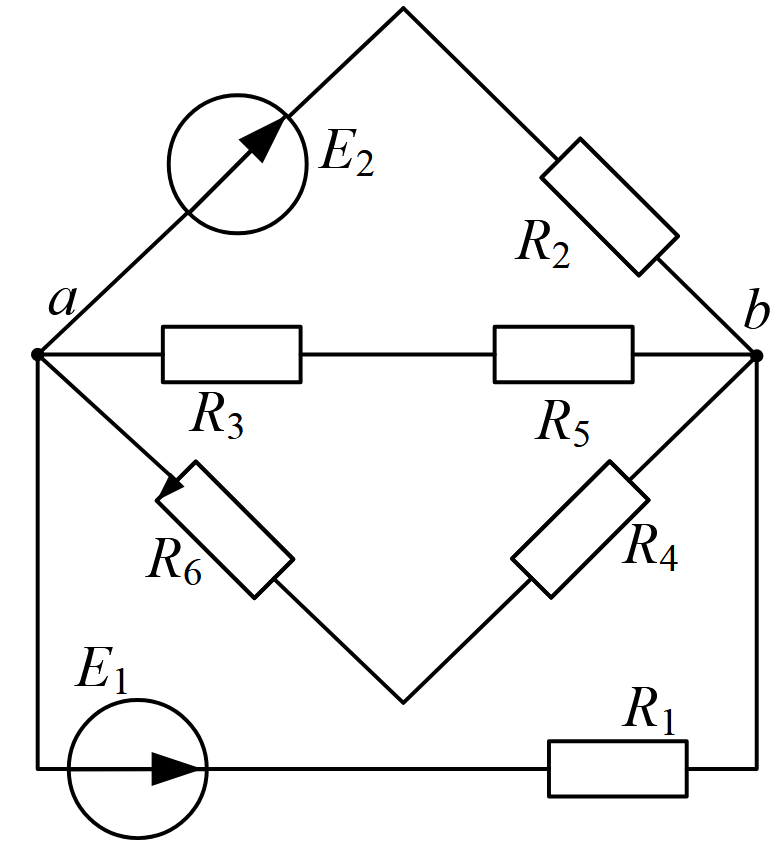
\includegraphics[width=\textwidth]{images/5_task.png}
        \caption{Вариант \#5}
        \label{fig:task_5}
    \end{minipage}
    \hfill
    \begin{minipage}{0.48\textwidth}
        \centering
        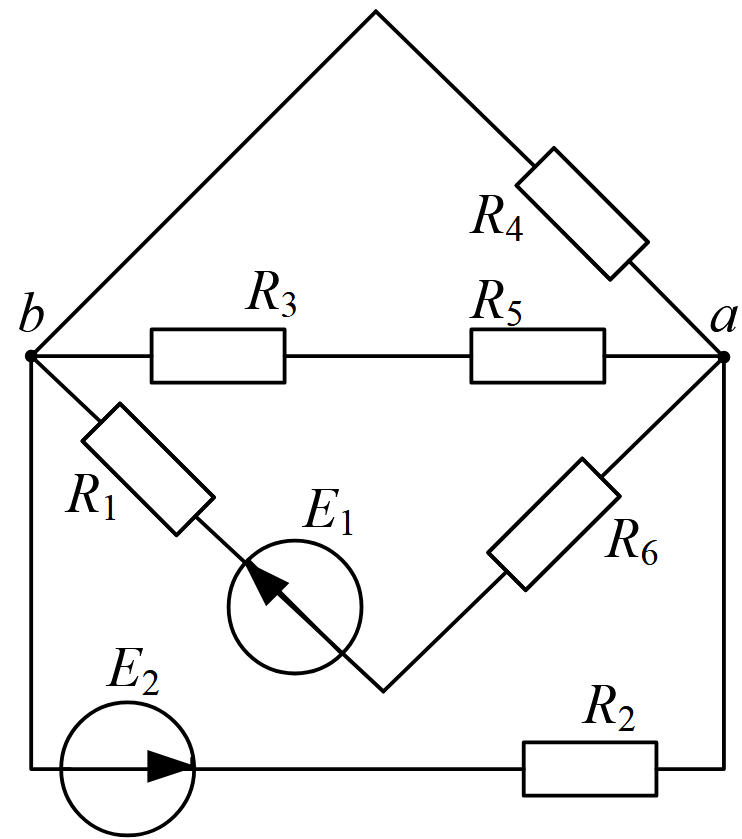
\includegraphics[width=\textwidth]{images/6_task.png}
        \caption{Вариант \#6}
        \label{fig:task_6}
    \end{minipage}
\end{figure}

% Ряд 4: Задачи 7-8
\begin{figure}[H]
    \centering
    \begin{minipage}{0.48\textwidth}
        \centering
        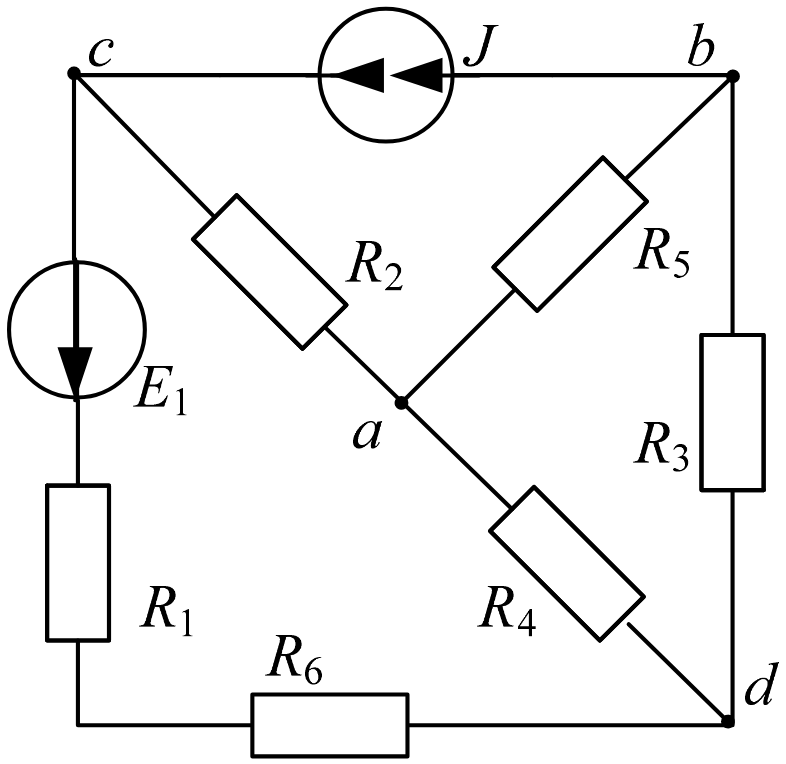
\includegraphics[width=\textwidth]{images/7_task.png}
        \caption{Вариант \#7}
        \label{fig:task_7}
    \end{minipage}
    \hfill
    \begin{minipage}{0.48\textwidth}
        \centering
        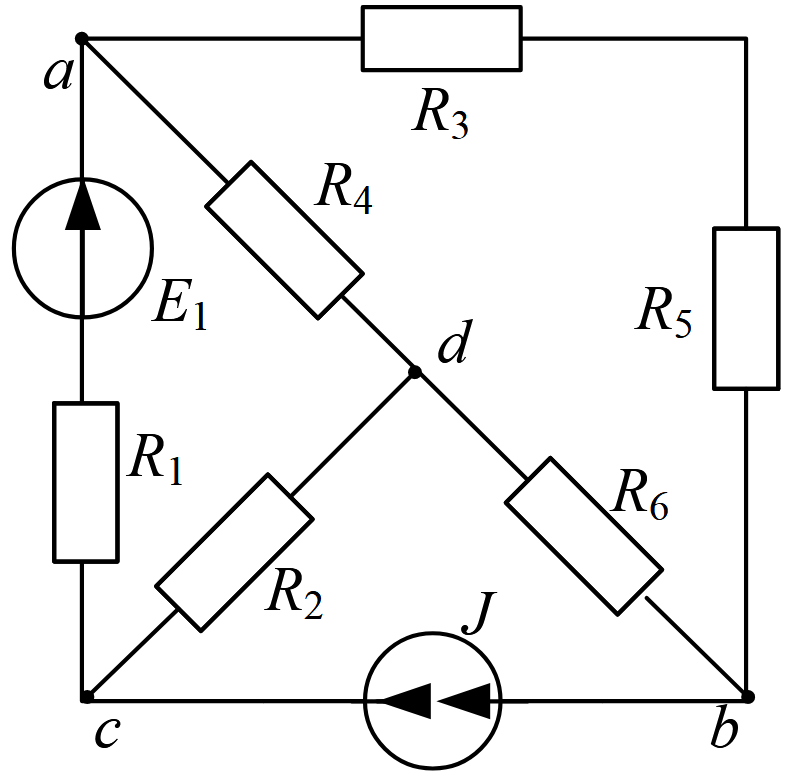
\includegraphics[width=\textwidth]{images/8_task.png}
        \caption{Вариант \#8}
        \label{fig:task_8}
    \end{minipage}
\end{figure}

% Ряд 5: Задачи 9-10
\begin{figure}[H]
    \centering
    \begin{minipage}{0.48\textwidth}
        \centering
        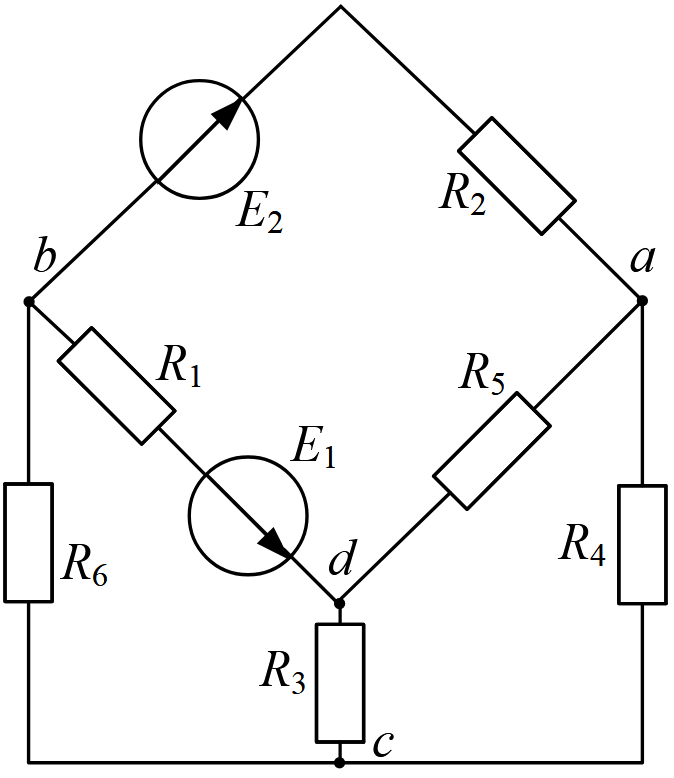
\includegraphics[width=\textwidth]{images/9_task.png}
        \caption{Вариант \#9}
        \label{fig:task_9}
    \end{minipage}
    \hfill
    \begin{minipage}{0.48\textwidth}
        \centering
        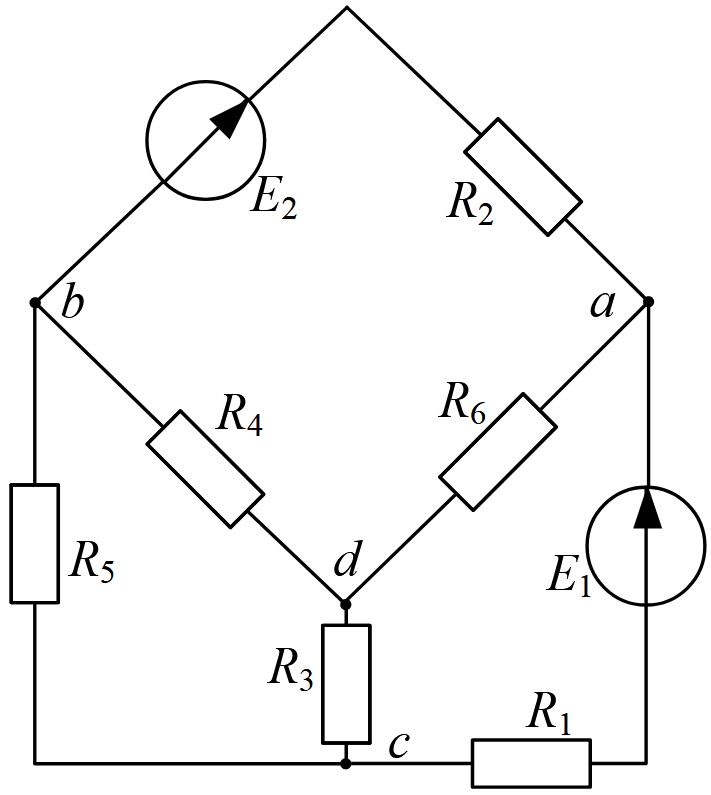
\includegraphics[width=\textwidth]{images/10_task.png}
        \caption{Вариант \#10}
        \label{fig:task_10}
    \end{minipage}
\end{figure}

% Ряд 6: Задачи 11-12
\begin{figure}[H]
    \centering
    \begin{minipage}{0.48\textwidth}
        \centering
        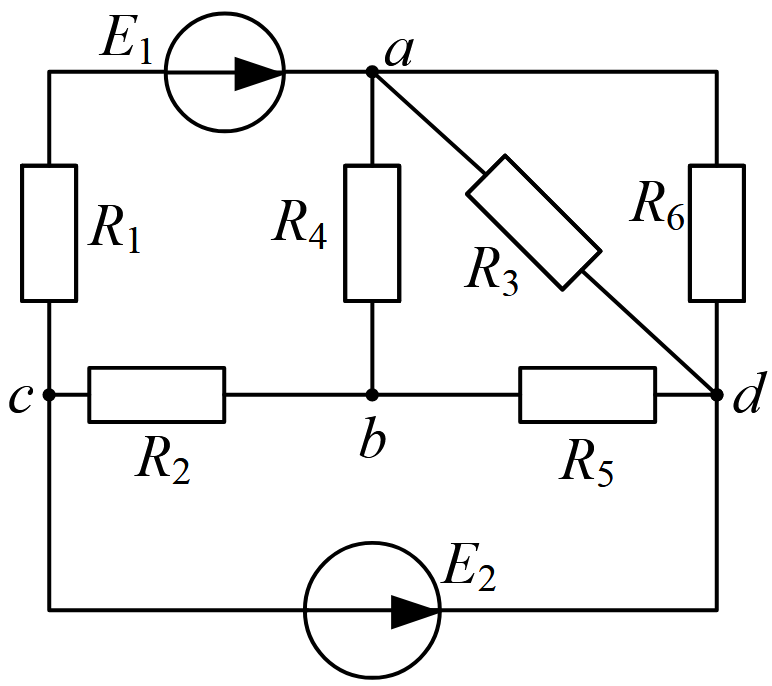
\includegraphics[width=\textwidth]{images/11_task.png}
        \caption{Вариант \#11}
        \label{fig:task_11}
    \end{minipage}
    \hfill
    \begin{minipage}{0.48\textwidth}
        \centering
        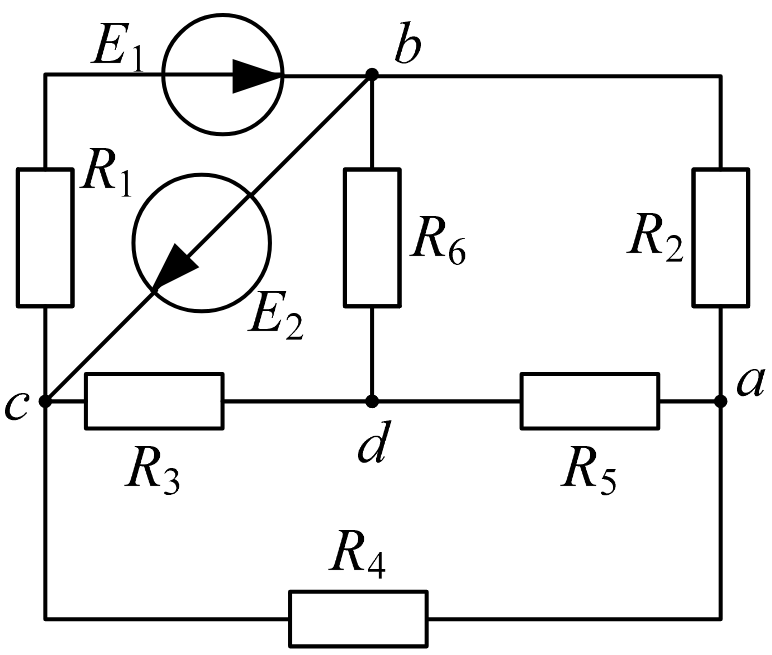
\includegraphics[width=\textwidth]{images/12_task.png}
        \caption{Вариант \#12}
        \label{fig:task_12}
    \end{minipage}
\end{figure}

% Ряд 7: Задачи 13-14
\begin{figure}[H]
    \centering
    \begin{minipage}{0.48\textwidth}
        \centering
        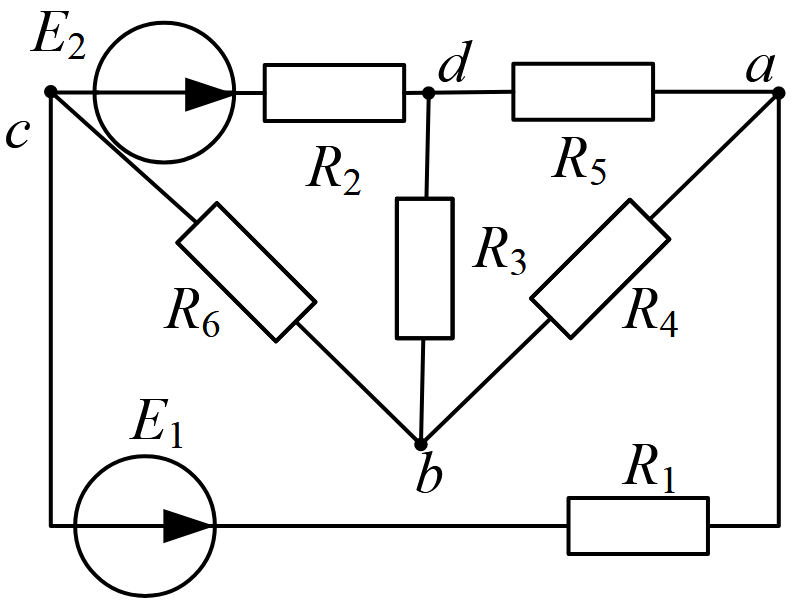
\includegraphics[width=\textwidth]{images/13_task.png}
        \caption{Вариант \#13}
        \label{fig:task_13}
    \end{minipage}
    \hfill
    \begin{minipage}{0.48\textwidth}
        \centering
        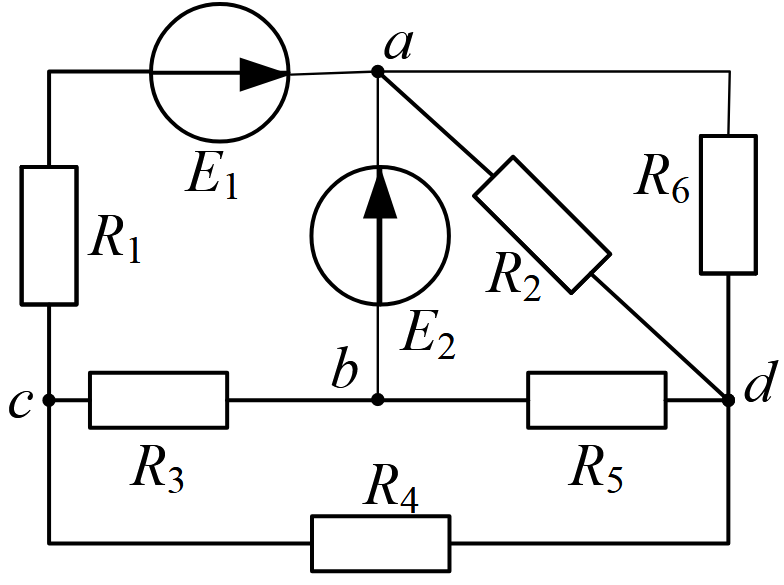
\includegraphics[width=\textwidth]{images/14_task.png}
        \caption{Вариант \#14}
        \label{fig:task_14}
    \end{minipage}
\end{figure}

% Ряд 8: Задачи 15-16
\begin{figure}[H]
    \centering
    \begin{minipage}{0.48\textwidth}
        \centering
        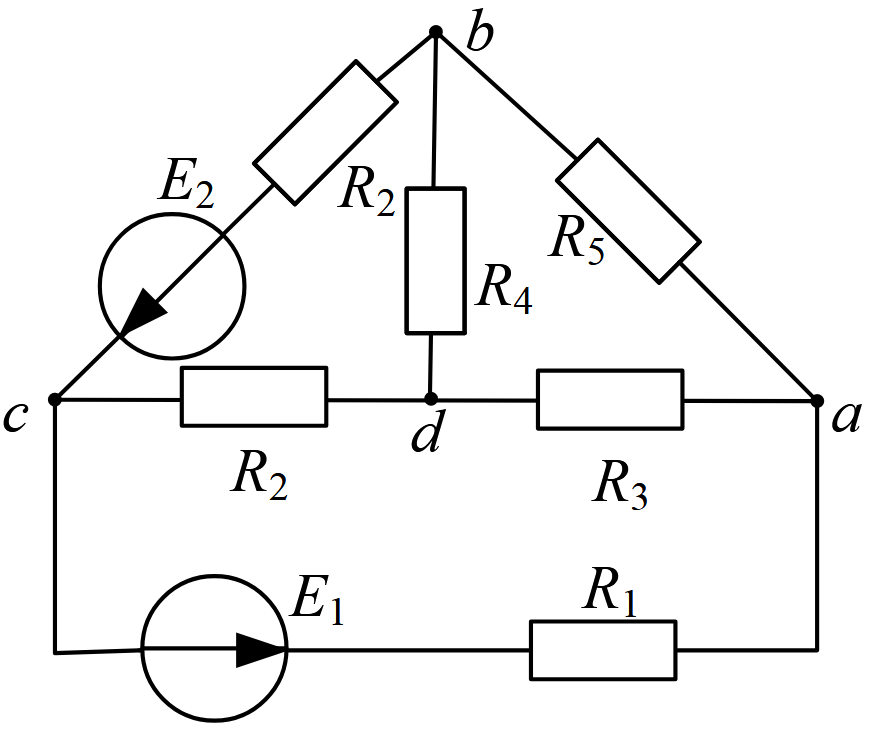
\includegraphics[width=\textwidth]{images/15_task.png}
        \caption{Вариант \#15}
        \label{fig:task_15}
    \end{minipage}
    \hfill
    \begin{minipage}{0.48\textwidth}
        \centering
        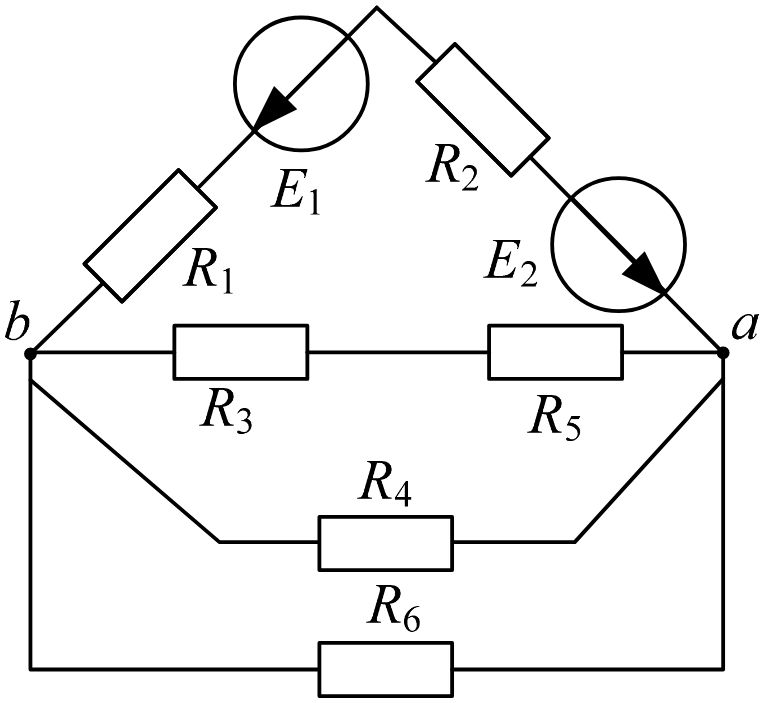
\includegraphics[width=\textwidth]{images/16_task.png}
        \caption{Вариант \#16}
        \label{fig:task_16}
    \end{minipage}
\end{figure}

% Ряд 9: Задачи 17-18
\begin{figure}[H]
    \centering
    \begin{minipage}{0.48\textwidth}
        \centering
        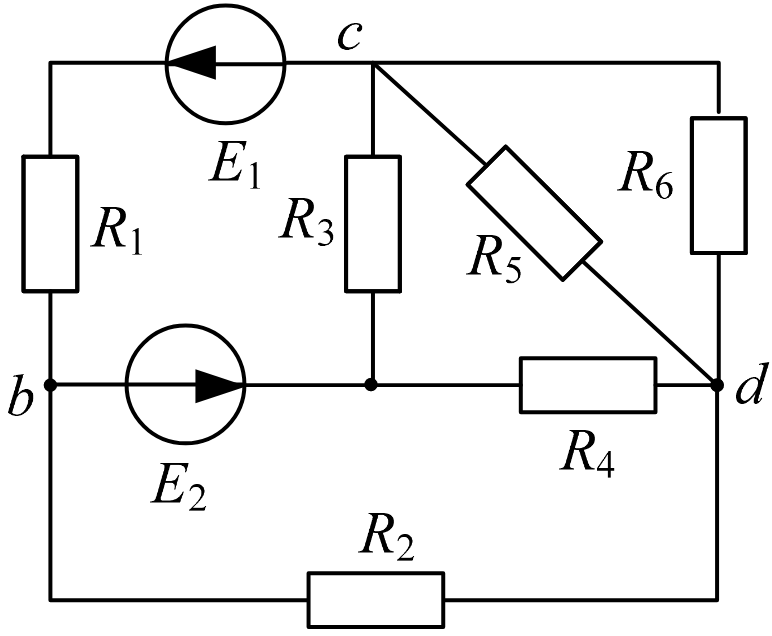
\includegraphics[width=\textwidth]{images/17_task.png}
        \caption{Вариант \#17}
        \label{fig:task_17}
    \end{minipage}
    \hfill
    \begin{minipage}{0.48\textwidth}
        \centering
        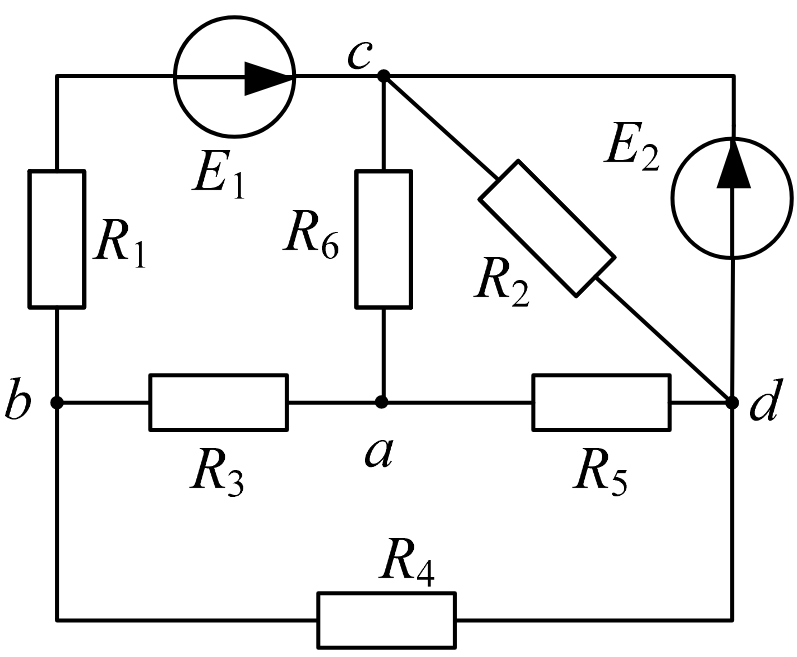
\includegraphics[width=\textwidth]{images/18_task.png}
        \caption{Вариант \#18}
        \label{fig:task_18}
    \end{minipage}
\end{figure}

% Ряд 10: Задачи 19-20
\begin{figure}[H]
    \centering
    \begin{minipage}{0.48\textwidth}
        \centering
        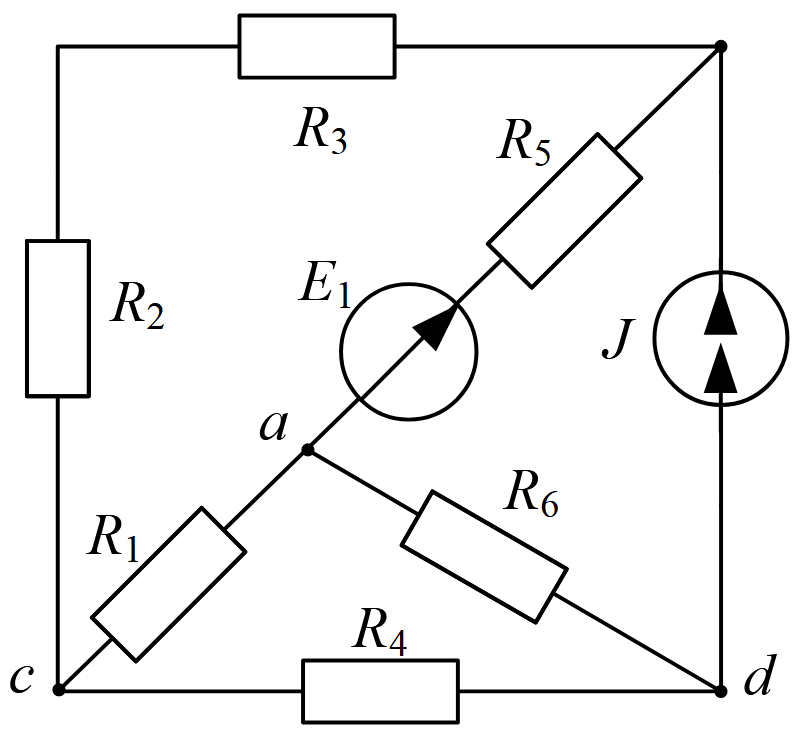
\includegraphics[width=\textwidth]{images/19_task.png}
        \caption{Вариант \#19}
        \label{fig:task_19}
    \end{minipage}
    \hfill
    \begin{minipage}{0.48\textwidth}
        \centering
        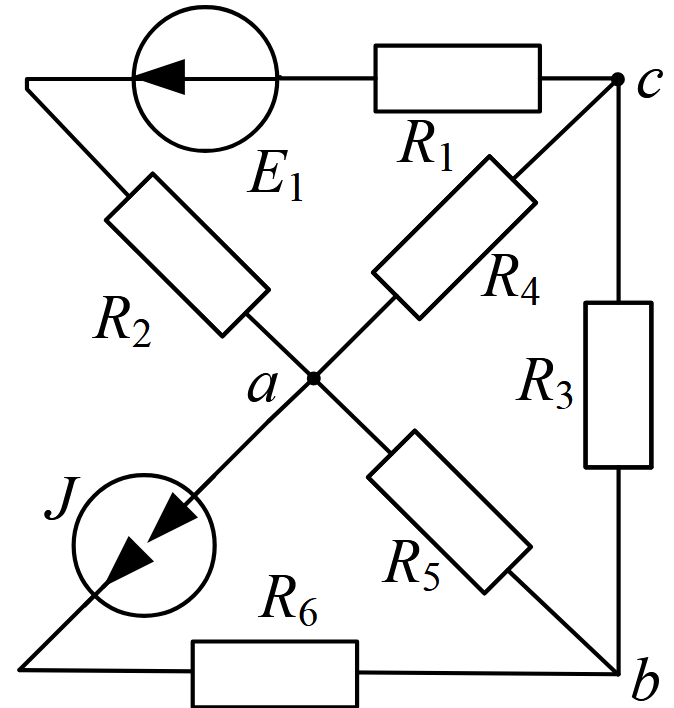
\includegraphics[width=\textwidth]{images/20_task.png}
        \caption{Вариант \#20}
        \label{fig:task_20}
    \end{minipage}
\end{figure}

% Ряд 11: Задачи 21-22
\begin{figure}[H]
    \centering
    \begin{minipage}{0.48\textwidth}
        \centering
        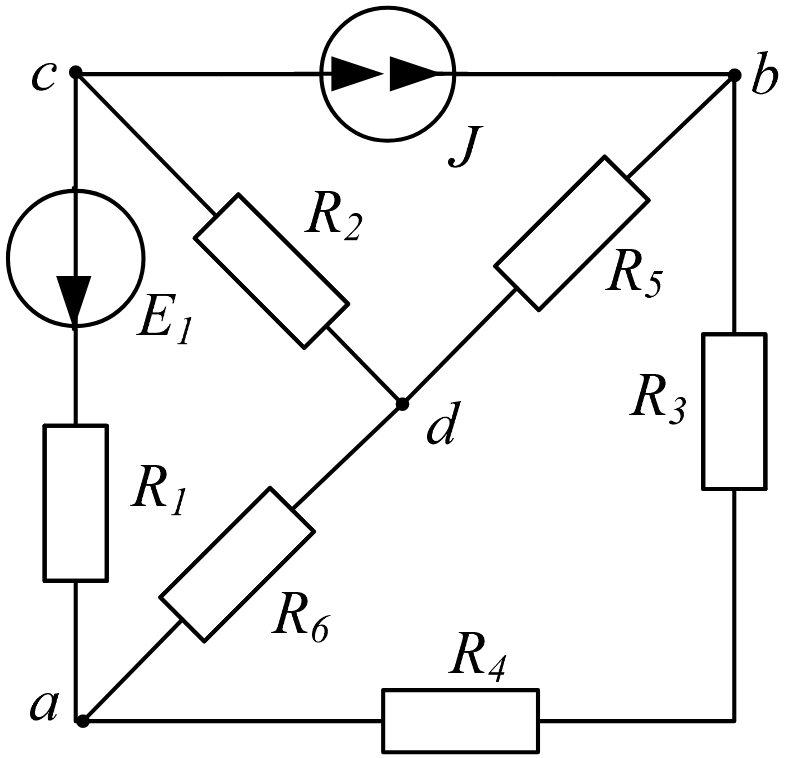
\includegraphics[width=\textwidth]{images/21_task.png}
        \caption{Вариант \#21}
        \label{fig:task_21}
    \end{minipage}
    \hfill
    \begin{minipage}{0.48\textwidth}
        \centering
        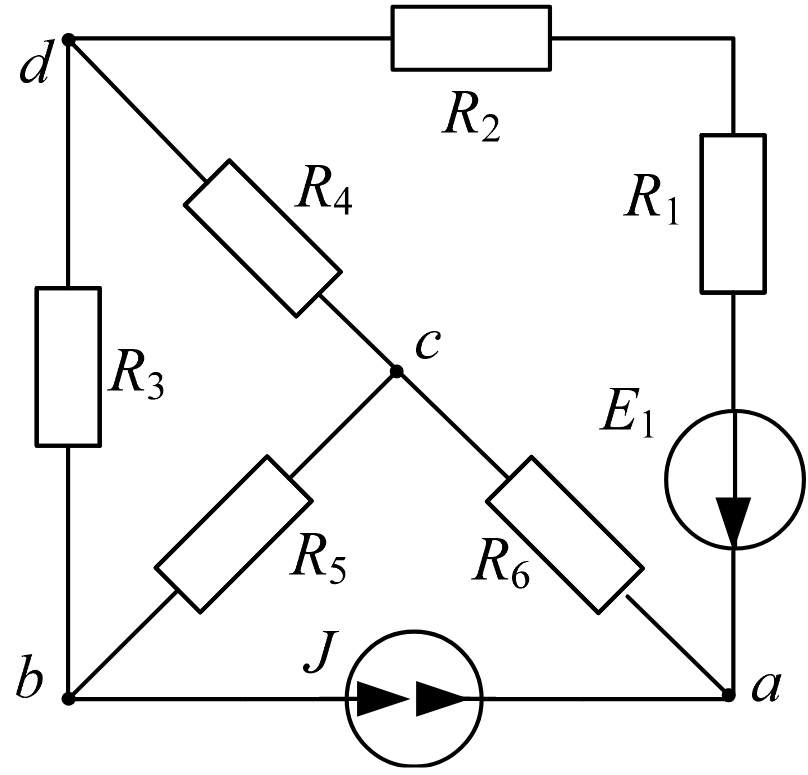
\includegraphics[width=\textwidth]{images/22_task.png}
        \caption{Вариант \#22}
        \label{fig:task_22}
    \end{minipage}
\end{figure}

% Ряд 12: Задачи 23-24
\begin{figure}[H]
    \centering
    \begin{minipage}{0.48\textwidth}
        \centering
        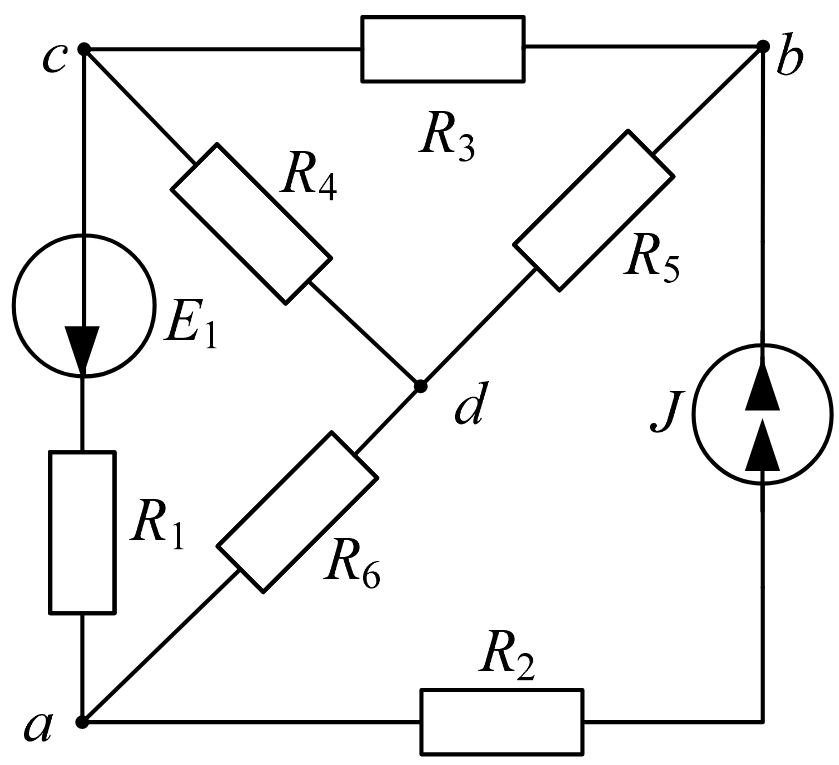
\includegraphics[width=\textwidth]{images/23_task.png}
        \caption{Вариант \#23}
        \label{fig:task_23}
    \end{minipage}
    \hfill
    \begin{minipage}{0.48\textwidth}
        \centering
        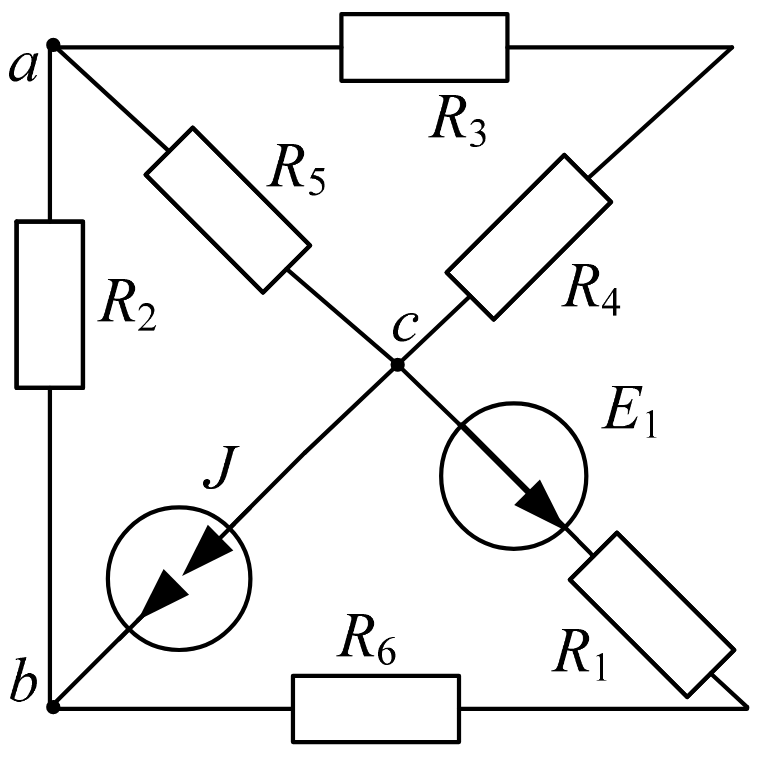
\includegraphics[width=\textwidth]{images/24_task.png}
        \caption{Вариант \#24}
        \label{fig:task_24}
    \end{minipage}
\end{figure}

% Ряд 13: Задачи 25-26
\begin{figure}[H]
    \centering
    \begin{minipage}{0.48\textwidth}
        \centering
        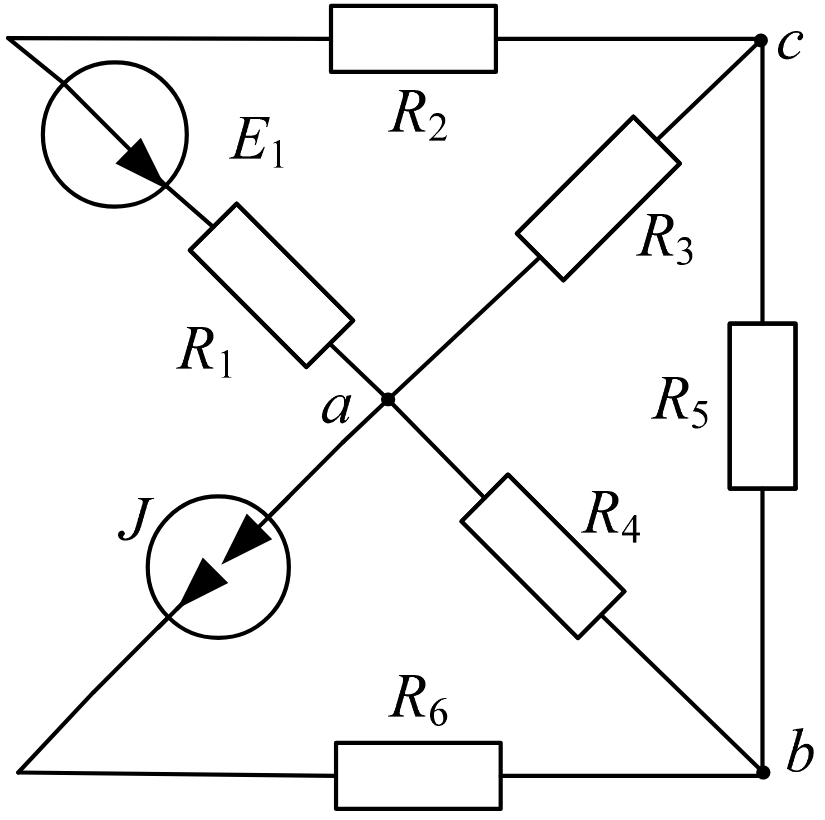
\includegraphics[width=\textwidth]{images/25_task.png}
        \caption{Вариант \#25}
        \label{fig:task_25}
    \end{minipage}
    \hfill
    \begin{minipage}{0.48\textwidth}
        \centering
        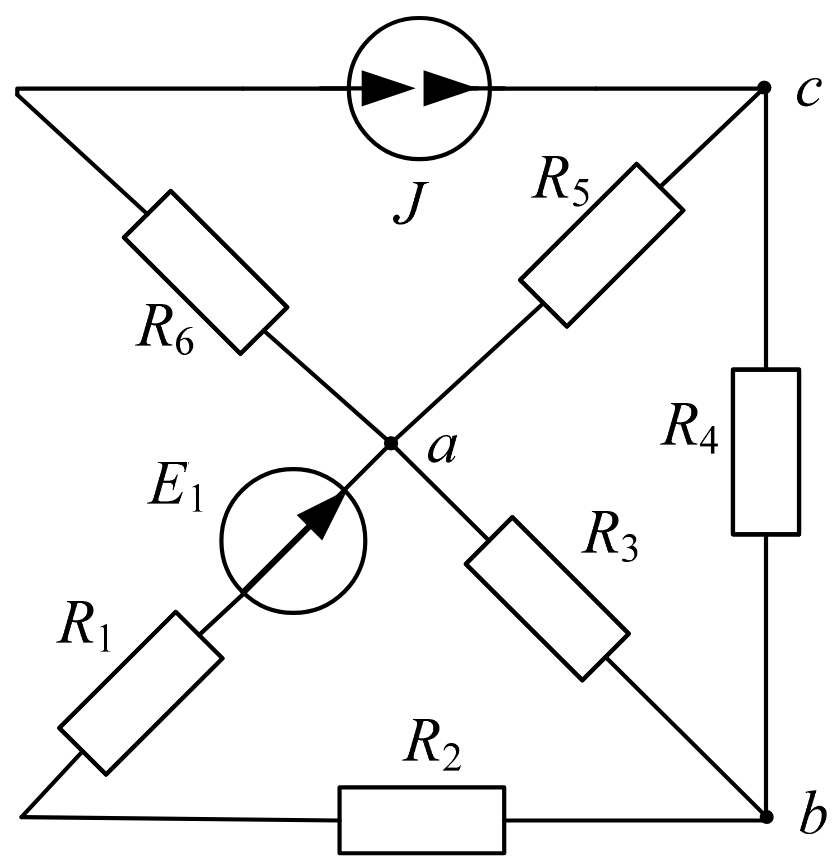
\includegraphics[width=\textwidth]{images/26_task.png}
        \caption{Вариант \#26}
        \label{fig:task_26}
    \end{minipage}
\end{figure}

% Ряд 14: Задачи 27-28
\begin{figure}[H]
    \centering
    \begin{minipage}{0.48\textwidth}
        \centering
        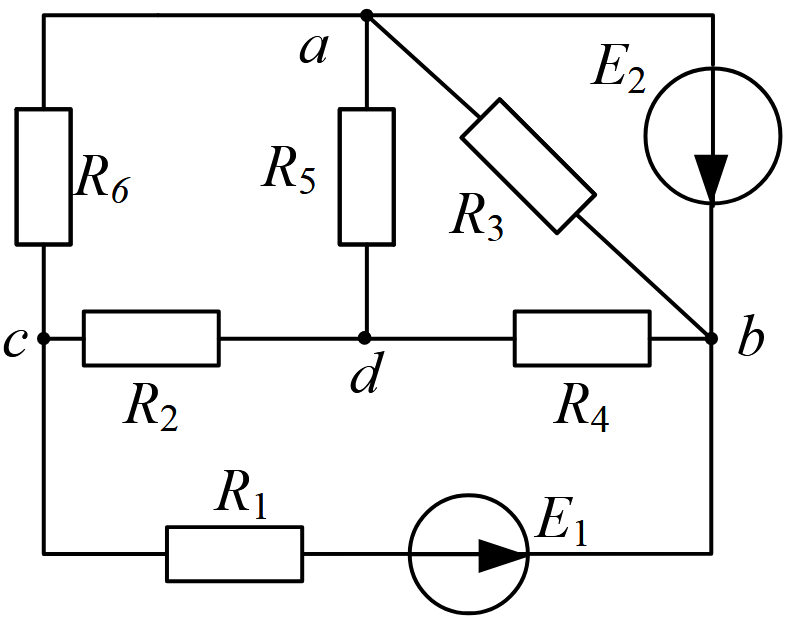
\includegraphics[width=\textwidth]{images/27_task.png}
        \caption{Вариант \#27}
        \label{fig:task_27}
    \end{minipage}
    \hfill
    \begin{minipage}{0.48\textwidth}
        \centering
        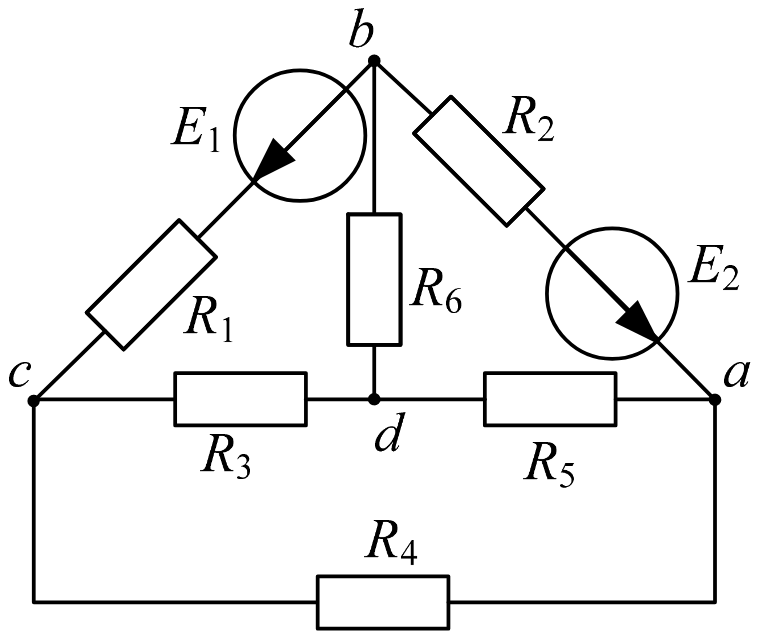
\includegraphics[width=\textwidth]{images/28_task.png}
        \caption{Вариант \#28}
        \label{fig:task_28}
    \end{minipage}
\end{figure}


